\documentclass[a4paper,12pt]{article}

% --- Pacotes essenciais ---
\usepackage[utf8]{inputenc}   % Codificação de caracteres
\usepackage[T1]{fontenc}      % Acentos corretos
\usepackage[brazil]{babel}    % Idioma português do Brasil
\usepackage{booktabs}         % Linhas mais elegantes nas tabelas
\usepackage{caption}          % Melhor controle sobre legendas
\usepackage{geometry}         % Controle de margens
\usepackage{array}            % Controle de largura das colunas
\usepackage{multirow}         % Combinar células verticalmente
\usepackage{float}            % Permite usar [H] para fixar tabelas
\usepackage{siunitx}          % Alinhamento numérico e formatação de números
\usepackage{pgfplots}
\pgfplotsset{compat=1.18}
% --- Configurações de layout ---
\geometry{a4paper, margin=2.5cm}
\captionsetup{justification=centering, font=small}

% --- Formatação de números decimais opcional, vírgula como separador ---
\sisetup{
  output-decimal-marker = {,}
}

\begin{document}

Apresentamos de forma simplificada os códigos desenvolvidos em GNU Octave para a obtenção dos pontos umbílicos discretos, das características robustas, das curvaturas Gaussiana discreta, média discreta, principais discretas e direções principais discretas. 

Nós usamos um computador com 1.6 GHz 8-Core com processador Intel Core i5 e 8 GB de memória e para a criação dos códigos e as computações realizadas utilizamos a versão 4.4.0 do GNU Octave para o sistema operacional Debian 10.


Foram desenvolvidos dois códigos principais:  ``parabolicafinal.m'' (que encontra as curvas parabólicas discretas) e ``ridgesesubparabolicafinal.m'' (que identifica apenas as curvas ridges discretas ou ambas, as curvas ridges e as curvas subparabólicas discretas), além de códigos auxiliares que calculam a área de faces, ângulos internos de faces, vetores normais de faces, entre outros.

As curvas ridges e as curvas subparabólicas discretas são obtidas no mesmo programa, uma vez que os pontos umbílicos discretos encontrados são usados para ambas as curvas. Ao iniciar o código, é possível escolher se o programa calculará ambas as curvas ou apenas as curvas ridges.

A parte inicial dos códigos principais é idêntica e segue o esquema representado na Figura \ref{esqcod}.

O código inicia com a leitura do arquivo .obj, que contém as coordenadas dos vértices e os índices dos vértices que formam cada uma das faces da triangulação da superfície linear por partes. A Tabela \ref{obj} apresenta um exemplo de um arquivo .obj no formato adequado para a leitura pelo código.

\begin{figure}[H] 
	\begin{center} 
		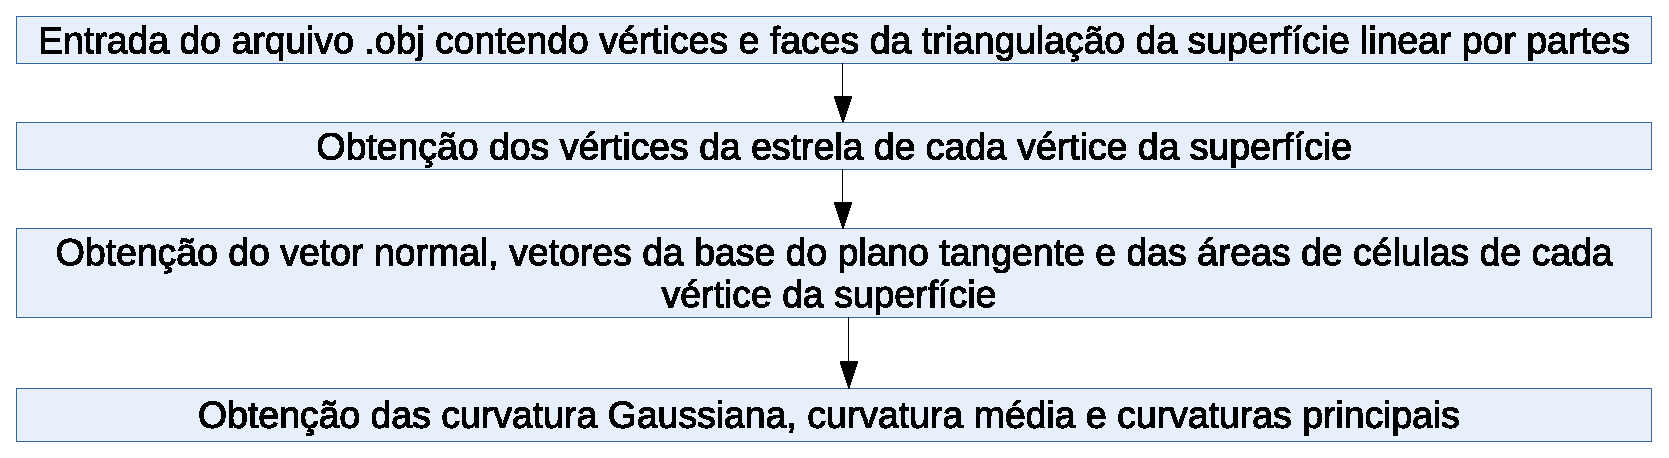
\includegraphics[angle=0,scale=0.56]{fig1.eps} 
		%\vspace{-0.5cm}
		    \caption{Etapas para a obtenção das curvatura Gaussiana discreta, curvatura média discreta e curvaturas principais discretas. Fonte: Elaborada pelo autor.} \label{esqcod}
		 \end{center} 
\end{figure}



\begin{table}[H]
\centering
\begin{tabular}{l}
\hline
v 1.000000 0.000000 2.000000 \\
v 2.761062 0.000000 8.623462 \\
v 4.522124 0.000000 21.449601 \\
v 6.283185 0.000000 40.478418 \\
v -0.500000 0.866025 2.000000 \\
v -1.380531 2.391150 8.623462 \\
v -2.261062 3.916274 21.449601 \\
v -3.141593 5.441398 40.478418 \\
v -0.500000 -0.866025 2.000000 \\
v -1.380531 -2.391150 8.623462 \\
v -2.261062 -3.916274 21.449601 \\
v -3.141593 -5.441398 40.478418 \\
v 1.000000 -0.000000 2.000000 \\
v 2.761062 -0.000000 8.623462 \\
v 4.522124 -0.000000 21.449601 \\
v 6.283185 -0.000000 40.478418 \\
f 1 5 6 \\
f 1 6 2 \\
f 5 9 10 \\
f 5 10 6 \\
f 9 13 14 \\
f 9 14 10 \\
f 2 6 7 \\
f 2 7 3 \\
f 6 10 11 \\
f 6 11 7 \\
f 10 14 15 \\
f 10 15 11 \\
f 3 7 8 \\
f 3 8 4 \\
f 7 11 12 \\
f 7 12 8 \\
f 11 15 16 \\
f 11 16 12 \\
\hline
\end{tabular}
\caption{Exemplo de arquivo .obj. Fonte: Elaborada pelo autor.} \label{obj}
\end{table}

Em seguida, identificamos os vértices $v_j$ da estrela de cada vértice $v_i$ da triangulação, a quantidade de vértices na estrela e as faces a que cada vértice $v_i$ pertence.

\begin{obs} 
Para a obtenção das curvas ridges e subparabólicas discretas, é fundamental que os vértices $v_j$ das estrelas de $v_i$  estejam organizados de forma sequencial, permitindo o cálculo de $\varphi_{v_iv_j}$. Neste código, os vértices das estrelas foram dispostos no sentido anti-horário. Por exemplo, para o vértice $v_6$ apresentado na Figura \ref{exestrela}, o programa fornecerá a estrela na seguinte ordem: $v_1,v_5,v_{10},v_{11},v_7,v_2$,  ou em uma sequência obtida por rotação dessa disposição.

\begin{figure}[h] 
	\begin{center} 
		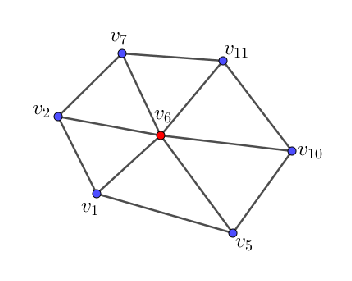
\includegraphics[angle=0,scale=1.0]{fig3.eps} 
		%\vspace{-0.5cm}
		    \caption{Obtenção da estrela do vértice $v_6$ de forma sequencial. Fonte: Elaborada pelo autor.} \label{exestrela}
		 \end{center} 
\end{figure}
\end{obs}

No terceiro passo, calculamos os vetores normais em cada vértice, os vetores da base do plano tangente em cada vértice (necessários para a obtenção das curvas ridges e subparabólicas discretas) e as áreas das células associadas a cada vértice da superfície.

Por fim, determinamos as curvaturas Gaussianas discretas, as curvaturas médias discretas e as curvaturas principais discretas em cada vértice da superfície.

Com as curvaturas Gaussianas discretas, curvaturas médias discretas e curvaturas principais discretas calculadas em cada vértice da superfície, é possível identificar os seguintes pontos: umbílicos discretos, parabólicos discretos, ridges discretos e subparabólicos discretos.

\section{Exibição das curvas parabólicas}

Conhecidos os pontos parabólicos, no programa ``parabolicafinal.m'', presentes na variável `MM', o próximo passo é traçar as curvas parabólicas discretas. 

Para obtermos os pontos ordenados de cada curva discreta, utilizamos duas variáveis:

\begin{itemize}
\item \textbf{Variável `jafoi':} uma matriz coluna com o mesmo número de linhas que `MM'. Esta variável indica se o ponto $P_i$, linha $i$ da matriz `MM', já foi utilizado ou não em alguma curva. Se na linha $i$ temos valor 0, indica que $P_i$ é um ponto não utilizado, se tivermos 1, indica que $P_i$ é um ponto utilizado.

\item \textbf{Variável `MM2':} uma matriz com 3 colunas, inicialmente. Nesta matriz, serão colocados os pontos ordenados de cada curva parabólica encontrada.
\end{itemize}

O programa realiza dois processos:

\begin{itemize}
\item[1)] \textbf{Inicialização:} O programa inicia com o ponto parabólico inicial, que chamaremos de $P_1$​, localizado na primeira linha da matriz `MM'. Marcamos a linha $1$ como visitada na variável `jafoi' e registramos as coordenadas de $P_1$ na primeira linha da matriz `MM2'.  

Em seguida, busca-se outro ponto parabólico $P_2$, ainda não visitado,   pertencente à mesma face do ponto $P_1$. Quando $P_2$ é encontrado, marcamos a linha $i$ de $P_2$ como visitada na variável `jafoi' e registramos suas coordenadas na segunda linha da matriz `MM2'. 

Posteriormente, busca-se um próximo ponto parabólico $P_{3}$, ainda não visitado,  que também esteja na mesma face do ponto $P_2$. Quando $P_{3}$ é encontrado, marcamos a linha $j$ de $P_{3}$ como visitada na variável `jafoi' e e registramos suas coordenadas na terceira linha da matriz `MM2'.

Esse processo continua iterativamente, buscando o ponto parabólico $P_{k}$, ainda não visitado, na mesma face do ponto $P_{k-1}$. O ciclo se encerra quando nenhum novo ponto $P_{l}$,  não visitado, puder ser encontrado na mesma face.

Após o término da primeira iteração, o processo é repetido, reiniciando-se no primeiro ponto $P$ ainda não visitado da matriz `MM'. Os pontos identificados nesta nova iteração são registrados na matriz `MM2', começando na linha 1 e na coluna $3t+1$, onde $t$ representa o número de vezes que o processo foi reiniciado. O procedimento continua até que todos os pontos de `MM' tenham sido visitados.

Desta forma, o número de colunas da matriz `MM2', dividido por 3, corresponde à quantidade de curvas parabólicas $h$ na superfície. Os pontos de cada curva estão distribuídos nas colunas de `MM2' como segue: colunas 1 a 3, 4 a 6, $\ldots$, $3h-2$ a $3h$.  

\item[2)] \textbf{Detectando curvas fechadas:} Após determinar as curvas, o programa verifica se cada curva é uma curva fechada. Como não há repetição de pontos durante a obtenção das curvas, o programa verifica se o primeiro e o último ponto de cada curva pertencem à mesma face. Se essa condição for satisfeita, a curva é considerada fechada, e o programa adiciona o primeiro ponto ao final da curva, garantindo que, ao traçar as curvas, elas sejam representadas como fechadas.
\end{itemize}

Por fim, o programa verifica a quantidade de curvas parabólicas abertas e fechadas obtidas na superfície e realiza o traçado das curvas parabólicas identificadas.

\section{Exibição das curvas ridges}

Detalharemos aqui o funcionamento do programa ``ridgesesubparabolicafinal.m''. 

Após o encontro das curvaturas, primeiramente, o programa encontra com as curvas ridges e os pontos umbílicos (detalhado na \autoref{section:secaoumb}). 

Os pontos ridges azuis em arestas são armazenados na variável `MM', enquanto os pontos ridges vermelhos em arestas são armazenados na variável `MMw'. Além disso, os vértices que são ridges azuis são armazenados na variável `zero', e os vértices que são ridges vermelhos, na variável `zero2'.


Diferentemente do programa ``parabolicafinal.m'', que requer apenas dois passos para encontrar as curvas parabólicas após os pontos parabólicos serem identificados, o processo para determinar as curvas ridges exige 10 passos adicionais após os pontos ridges (azuis e vermelhos) serem encontrados. Apresentamos o procedimento para as curvas ridges azuis; para as ridges vermelhas o processo é o mesmo.

\begin{itemize}
\item[1)] \textbf{Inicialização:} Este passo é idêntico ao primeiro passo das curvas parabólicas. As curvas ridges azuis são armazenadas na variável  `MM2' (as curvas ridges vermelhas, na variável `MM2w').

\item[2)] \textbf{Junção de curvas iniciais:} O programa junta duas curvas ridges azuis cujo primeiro ponto da curva 1 e o primeiro ponto da curva 2 estão na mesma face.

\item[3)] \textbf{Junção de extremos:} O programa junta duas curvas ridges azuis cujo último ponto da curva 1 e o primeiro ponto da curva 2 estão na mesma face.

\item[4)] \textbf{Passagem por vértices intermediários (último ponto):} O programa ajusta a curva ridge azul para que, se o último ponto da curva estiver na mesma face de um vértice que também é ridge azul, a curva passe por esse vértice.

\item[5)] \textbf{Passagem pelo ponto umbílico:} O programa ajusta as curvas ridges azuis para garantir que elas passem pelos pontos umbílicos, conforme \autoref{section:secaoumb}.

\item[6)] \textbf{Passagem por vértices intermediários (primeiro ponto):} O programa ajusta a curva ridge azul para que, se o primeiro ponto da curva estiver na mesma face de um vértice que também é ridge azul, a curva passe por esse vértice.

\item[7)] \textbf{Fusão de curvas adjacentes (últimos pontos):} Junta-se duas curvas ridges azuis cujo último ponto da curva 1 e o primeiro ponto da curva 2 são os mesmos.

\item[8)] \textbf{Fusão de curvas adjacentes (primeiros pontos):} Junta-se duas curvas ridges azuis cujo primeiro ponto da curva 1 e o primeiro ponto da curva 2 são os mesmos.

\item[9)] \textbf{Análise dos pontos umbílicos:} O programa verifica se todos os pontos umbílicos possuem curvas ridge azuis passando por eles. Há dois casos em que pode não haver uma curva ridge passando por um ponto umbílico: o primeiro ocorre quando há uma curva ridge fechada inteiramente na estrela do ponto umbílico; o segundo ocorre quando o ponto umbílico se originou de dois pontos umbílicos, vértices de uma mesma aresta, ou seja, o ponto umbílico final é o ponto médio desses dois pontos, como detalhado na \autoref{section:secaoumb}. Neste caso, o programa realiza uma correção na escolha do ponto umbílico, ajustando para considerar o outro ponto que havia sido descartado.

\begin{obs}
\begin{itemize} 
\item[a)] O índice dos pontos umbílicos que não possuem curva ridge azul passando por eles, pois havia uma curva ridge fechada inteiramente na estrela é indicado no código ``ridgesesubparabolicafinal.m'' pela variável `pontodegenerado' e, para obter suas coordenadas, basta utilizar o comando `Pumbc(pontodegenerado,:)'. 
\item[b)] Nas curvas ridges vermelhas, verificamos apenas se há ponto umbílico sem curvas ridges vermelhas passando por ele, o índice desse ponto umbílico é indicado no código pela variável `pontodegeneradow', sem executar a segunda parte do passo, para evitar retornar ao ponto inicial.
\end{itemize}

\end{obs}

Após esse passo, o programa retorna ao Passo 2 e refaz os passos de 2 a 8 até que não haja mais mudanças nas curvas.

\item[10)] \textbf{Detectando curvas fechadas:} Após determinar as curvas, o programa verifica se cada curva ridge é fechada. Este processo é idêntico ao passo correspondente das curvas parabólicas. 
\end{itemize}

A seguir, o programa determina as curvas ridges vermelhas e verifica a quantidade de curvas ridges abertas e fechadas obtidas na superfície.


Caso estejamos analisando uma face obtida por meio da triangulação realizada com o MediaPipe, o programa verifica a quais regiões da face cada ponto umbílico pertence, indicando tanto a região quanto a quantidade de pontos umbílicos em cada uma. Para isso, é necessário ativar essa funcionalidade no código.

\section{Exibição das curvas subparabólicas}


Iniciamos o processo para determinar as curvas subparabólicas. Os pontos subparabólicos vermelhos são armazenados na variável `MMs', enquanto os pontos subparabólicos azuis são armazenados na variável `MMsw'. Além disso, os vértices que são subparabólicos vermelhos são armazenados na variável `zerosub', e os vértices que são subparabólicos azuis, na variável `zerosub2'.

O processo para determinar as curvas subparabólicas é idêntico ao realizado para as curvas ridges. Dos 10 passos apresentados anteriormente, realizamos todos, sendo que no Passo 9, verificamos apenas se há ponto umbílico sem curvas subparabólicas passando por ele. O índice desses pontos umbílicos são indicados no código pelas variáveis `pontodegenerados' (para a curva subparabólica vermelha) e `pontodegeneradosw' (para a curva subparabólica azul). No Passo 1, as curvas subparabólicas vermelhas são armazenadas na variável `MMs2' e as curvas subparabólicas azuis, na variável `MMs2w'.

Por fim, o programa verifica a quantidade de curvas subparabólicas abertas e fechadas obtidas na superfície.

Após determinar todas as curvas ridges e subparabólicas, o programa realiza o traçado das curvas identificadas. As curvas ridges azuis são traçadas na cor azul, as curvas ridges vermelhas na cor vermelha, as curvas subparabólicas vermelhas na cor magenta e as curvas subparabólicas azuis na cor ciano.

Para obter as curvas discretas, conhecidos os pontos ordenados  de cada curva, o programa traça as arestas utilizando os comandos `plot3' (gráficos em 3D) e `-' (gráficos contínuos).



\begin{obs}
As mensagens exibidas durante a execução do código, como Parte1, Parte2, ..., Parte8, Azul1, ..., Azul6, e Vermelha1, ..., Vermelha6, servem apenas para indicar em qual parte do código o programa está sendo executado. Essas etapas não correspondem aos passos apresentados anteriormente.
\end{obs}

Para maiores informações, consulte:

\url{https://www.teses.usp.br/teses/disponiveis/55/55134/tde-10092025-142838/pt-br.php}

\end{document}